\documentclass[11pt,titlepage]{article}
%\usepackage[notref]{showkeys}
\usepackage[reqno]{amsmath}
\usepackage{natbib}
\usepackage{amssymb}
\usepackage{epsfig}
\usepackage{comment}
\usepackage{url}
\usepackage[all]{xy}        
\usepackage{dcolumn}
\newcolumntype{.}{D{.}{.}{-1}}
\newcolumntype{d}[1]{D{.}{.}{#1}}
\usepackage{threeparttable,booktabs}
\usepackage{times}
\usepackage{vmargin}
\setpapersize{USletter}
\topmargin=0in
\usepackage[compact]{titlesec}  % small
%\usepackage{ajps}
\usepackage{times}


% Shortcuts
\renewcommand{\P}{\text{P}}
\newcommand{\MC}{\multicolumn}
\usepackage{calc}
\newcounter{hours}\newcounter{minutes}
\newcommand{\printtime}{%
  \setcounter{hours}{\time/60}%
  \setcounter{minutes}{\time-\value{hours}*60}%
  \thehours :\theminutes}
%
\title{The Balance Test Fallacy in Matching\\ Methods for Causal
  Inference\thanks{Our thanks to Alberto Abadie, Neal Beck, Alexis
    Diamond, Guido Imbens, Paul Rosenbaum, Don Rubin, and Jas Sekhon
    for many helpful comments; and the National Institutes of Aging
    (P01 AG17625-01), the National Science Foundation (SES-0318275,
    IIS-9874747, SES-0550873), and the Princeton University Committee
    on Research in the Humanities and Social Sciences for research
    support.}}

\author{Kosuke Imai\thanks{Assistant Professor, Department of
    Politics, Princeton University (Corwin Hall 041, Department of
    Politics, Princeton University, Princeton NJ 08544, USA;
    \texttt{http://Imai.Princeton.Edu}, \texttt{KImai@Princeton.Edu},
    (609) 258-6601).}
\and 
  Gary King\thanks{David Florence Professor of Government, Harvard
    University (Institute for Quantitative Social Science, Harvard
    University, 1737 Cambridge St., Cambridge MA 02138;
    \texttt{http://GKing.Harvard.Edu}, \texttt{King@Harvard.Edu},
    (617) 495-2027).}
\and 
  Elizabeth A.\ Stuart\thanks{Researcher, Mathematica Policy Research,
    Inc.\, (600 Maryland Ave., SW, Suite 550, Washington, DC, 20024,
    USA; \texttt{http://people.iq.harvard.edu/$\sim$estuart/},
    \texttt{elizabeth.stuart@gmail.com}).}}

\date{\today} 

\begin{document}\maketitle
%\baselineskip=1.57\baselineskip

\begin{abstract}
  Matching methods are widely used to adjust for nonrandom treatment
  assignment when making causal inferences.  In numerous articles
  across a diverse variety of academic fields that use matching,
  researchers evaluate the success of the procedure by conducting
  hypothesis tests, most commonly the $t$-test for the mean difference
  of each of the observed covariates between the treated and control
  groups. We demonstrate that these hypothesis tests are fallacious
  and discuss better alternatives.
\end{abstract}

Across academic fields, matching is a popular method of improving
causal inference by nonparametrically adjusting for control variables
\citep{Imbens04,Rosenbaum02}.  In this paper, we show that a common
approach used in evaluating the success of this method, based on
hypothesis tests for the difference between the treated and control
groups, is invalid.

The ultimate goal of matching and the associated analyses we consider
is estimating the average causal effect of a binary treatment
variable, $T$, on an outcome variable, $Y$.\footnote{Causal quantities
  of interest can be defined in a variety of other ways, including
  average treatment effect on the treated.  Our argument applies to
  any of these quantities.}  In observational studies, researchers
typically invoke the strong ignorability assumption \citep{RosRub83},
which then requires controlling for a vector of observed covariates
$X$.  Matching is used to nonparametrically adjust for nonrandom
treatment assignment, by dropping or repeating observations, so that
the relationship between $X$ and $T$ --- and thus the need for
subsequent parametric adjustments for $X$ --- are eliminated or
reduced.  Adjusting the sample introduces no bias so long as the
matching rule for doing this is a function of $X$ and $T$ and not $Y$.
Matching is not a method of estimation, and so any application of it
must be followed by such a method.  In the best case, the data after
matching satisfy
\begin{equation}
  \label{balance}
  \tilde p(X\mid T=1) = \tilde p(X\mid T=0),
\end{equation}
where $\tilde p$ is the empirical density of the observed data, rather
than a population density.\footnote{To be more specific, the empirical
  density is defined as $\tilde p(x) = \# \{ i\in \{1, 2, \dots, n \}:
  X_i = x \} / n$, for all $x$, where $\#A$ is the number of elements
  in the set $A$ and $n$ is the number of observations. } In this best
case, $T$ and $X$ are unrelated in the matched sample, and no further
adjustments for $X$ are necessary. Indeed, the average treatment
effect can be estimated by a simple difference in means of $Y$ between
the treated ($T=1$) and control ($T=0$) groups.  When the sample
relationship between $T$ and $X$ is reduced but not eliminated,
further adjustment for $X$ may be necessary, such as via the same
parametric methods as would have been used if matching had not been
used. Moreover, it has been shown that matching can effectively reduce
the model dependence of subsequent parametric analyses
\citep{HoImaKin06}.  The immediate goal of matching, then, is to
choose an algorithm that satisfies (\ref{balance}) as best as
possible.  Since methodological work on matching is growing fast, the
list of available matching algorithms from which to choose is also
growing.

Standard practice is for researchers to evaluate (\ref{balance}) for
the chosen algorithm by conducting $t$-tests for the difference in
means for each variable in $X$ between the treatment and control
groups, thus seemingly addressing at least one important aspect of a
high dimensional relationship.  (Other hypothesis tests are also
sometimes used to evaluate higher dimensional differences in
(\ref{balance}), but the same problems we describe below still
applies, and so for expository purposes we focus on the simpler
$t$-test.)

The practice of using hypothesis tests to evaluate balance is
widespread, and includes a large volume of otherwise high quality work
in economics \citep{MilFreMcH03,BlaSmi04,AgoDyn04,DehWah99,
  DehWah02,SmiTod05}, political science \citep{Imai05,SimHop05},
sociology \citep{LunSmi05}, psychology
\citep{HavNag05,HilWalBro05,YosMagBos03,JonDAgGon04,McCRidMor04},
education \citep{Crosnoe05,SchBuc03}, management science
\citep{FreMil04, Villalonga04,WanSchAvo05}, medicine
\citep{WanSchAvo05, MacRivJur06,LinPekWan06,ManTudDie06, PetRoeMul06,
  ShiLitPot06,SabCanGib05,PerUndZho00,AusMam06,AusMamStu05}, public
health \citep{NovReaRau06,ElBGilWu05,LauSmiSta00,BinBreEar05}, and
statistics \citep{LuZanHor01}.  Tables of $t$-tests and other
hypothesis tests for balance are used as a justification in these and
other published articles for the adequacy of the chosen matching
solution, and insignificant $t$-tests are used as a stopping rule
during research while maximizing balance in the search for the right
analysis from which to draw inferences.  This approach is problematic
for at least four reasons.

First, consider a data set on the School Dropout Demonstration
Assistance Program which sought to reduce dropout rates by a series of
school ``restructuring'' initiatives, including curriculum reform,
expanding teacher training, and others \citep{AgoDyn04,Stuart04}.  We
use a subset of these data that includes 428 students from a treated
school ($T=1$) and 434 from a control school ($T=0$).  The outcome
variable $Y$ is a test score (coded as a percentage), and $X$ includes
a variety of variables but we focus here only on the baseline math
test score.  Matching begins with the full data set and then
selectively deletes students until (\ref{balance}) is best satisfied
without losing too many observations.  Suppose instead that we choose
a matching algorithm that \emph{randomly} selects observations to
discard.  Clearly, this algorithm would not effect balance, or the
bias in the ultimate analysis that satisfying (\ref{balance}) is meant
to improve.  Yet, we can show that randomly deleting observations does
wonders according to the $t$-test.  To do this, we create a sequence
of matching solutions that randomly drop different numbers of control
observations (with results averaged over 5000 draws), and plot the
average results in the left graph of Figure \ref{f:randrop}.  The
horizontal axis in this figure reports the number of control units
randomly dropped, while the vertical axis gives the size of the
$t$-test.  We have shaded in the area below a $t$-test of 2, which is
the region in which results are conventionally referred to as
``statistical insignificant''.  The line on the plot clearly shows
that, according to the $t$-test, randomly dropping more control units
does an ``excellent'' job at achieving balance, reducing the statistic
from 3.7 to 1.6 in the figure.  This of course makes no sense at all.
\begin{figure}[t]
  \centering
  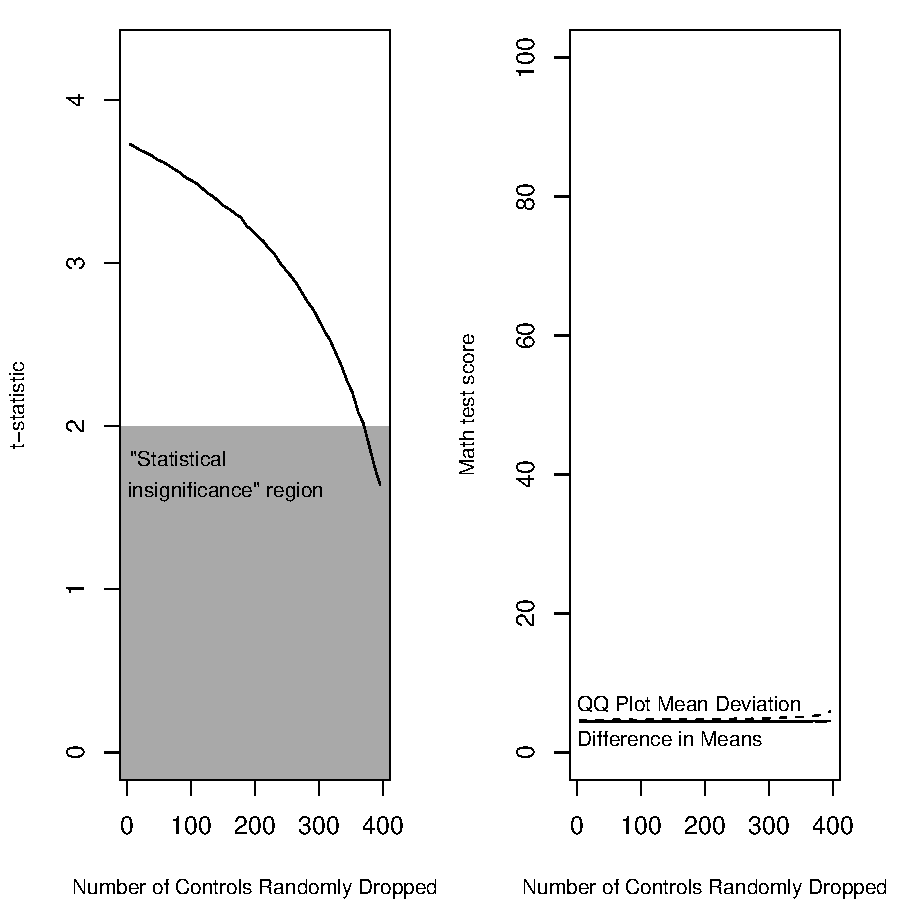
\includegraphics[height=4.5in]{figs/TStatPlotR0MATH}
  \caption{Dangers in relying on $t$-statistics as measure of balance.
    The solid lines in both graphs indicate the average value of a
    measure of balance when a given number of control units are
    randomly dropped from the data set (out of a total of 434).  With
    larger numbers of control units dropped (i.e., smaller numbers of
    control units in the resulting sample), the t-statistic gets
    closer to 0, falsely indicating improvements in balance, even
    though true balance does not vary systematically across the data
    sets (and efficiency declines).  The difference in means and QQ
    plot mean deviation, given in the right graph, correctly indicate
    no change in bias as observations are randomly dropped.}
  \label{f:randrop}
\end{figure}

Second, from a theoretical perspective, balance is a characteristic of
the sample, not some hypothetical population, and so strictly speaking
hypothesis tests are irrelevant in this context.  Virtually all
methods of adjustment condition on the observed values of $X$, and so
$X$ can be dropped in these analyses only when (\ref{balance}) is
satisfied in sample, not in some population from which the data are
hypothetically or actually drawn.  For the same reason that randomized
blocks are preferable to classical randomization in experimental
design --- that is, the bias that defines the blocks can be set to
zero in sample, without having to hope that the sample size is large
enough for the advantages of randomization to kick in --- matching on
all observables is preferable whenever feasible.  Indeed, in the best
case, we would be able to match exactly on all observables, and
afterwords randomize the assignment of values to the treatment
variable $T$.  That is, imbalance --- the difference between $\tilde
p(X\mid T=1)$ and $\tilde p(X\mid T=0)$ --- should be minimized
without limit where possible, so long as we are not compromising other
goals in the process (such as efficiency).

Third, we offer a simple model that conveys why matching contains no
de minimus level, below which the level of imbalance is acceptable.
To see this, consider data generated by the classical regression
model, $E(Y\mid X)= \theta + T\beta + X\gamma$ \citep{Goldberger91}.
Then the regression of $Y$ on a constant and $T$ (without $X$) gives a
difference in means, the bias of which as an estimate of $\beta$ is
$E(\hat\beta-\beta) = F\gamma$, where $F$ contains vectors of
coefficients of regressions of each of the variables in $X$ on a
constant and $T$.  Using matching to eliminate bias under this
simplified data generation process involves dropping or repeating
observations so that $F$ is as close to a matrix of zeros as possible.
But what happens to bias if $F$ is smaller than it was before matching
but still not zero?  The answer is that the bias is reduced, but
without knowledge of $\gamma$ --- which matching researchers eschew
estimating to ensure that they do not inadvertently introduce
selection bias by choosing matching solutions that stack the deck for
their favored hypotheses --- it could be that a nonzero portion of
$F$, when multiplied by $\gamma$, will generate arbitrarily large
bias.  Whether or not some hypothesis test indicates that $F$ is not
significantly different from zero is immaterial: The smaller $F$ is
the better, either above or below the $t$-test threshold of
significance, since $F$ (i.e., balance) is a characteristic of the
observed data.

Finally, the problem in Figure \ref{f:randrop} can be seen by
recognizing that dropping observations can influence not only balance
but also statistical power, and the $t$-test is unfortunately a
function of both.  The more observations dropped, the less power the
tests have to detect imbalance in observed covariates.  Formally, we
can write the two sample $t$-test statistic with unknown and
unequal variances as
\begin{equation}
  \label{ttest} \frac{\sqrt{n}(\overline{X}_t-\overline{X}_c)}
               {\sqrt{\frac{s^2_t}{r} + \frac{s^2_c}{1-r}}}
\end{equation}
where $s^2_t=\sum_{i=1}^n t_i(X_i - \overline{X}_t)^2/(n_t-1)$,
$s^2_c=\sum_{i=1}^n (1-t_i)(X_i - \overline{X}_t)^2/(n_c-1)$, $n_t$
and $n_c$ are the sample sizes for the treatment and control groups,
respectively, and $r=n_t/n$.  Hence, the difference in sample means as
a measure of balance is distorted in the $t$-test by three factors:
(1) the total number of remaining observations $n$, (2) the ratio of
remaining treated units to the total number of remaining observations
$r$, and (3) the variance of $X$ for the remaining treated and control
units, $s_t^2$ and $s_c^2$.  Since the value of (this and other)
hypothesis tests are affected by factors other than balance, they
cannot even be counted on to be monotonic functions of balance: The
$t$-test can indicate balance is getting better while the actual
balance is getting worse, staying the same, or improving.

Balance should thus be checked by comparing the observed covariate
differences between the treated and control groups and should be
minimized without limit.  A difference in means is a fine way to
start.  Statisticians tend to standardize the mean differences so the
measure can be compared across different variables.  This is a
reasonable approach used to simplify the analysis, but in our view the
standardization also makes the variables invariant to the substantive
research question (and to priors about likely values of $\gamma$ or
the equivalent).  A more general approach are quantile-quantile (or
``QQ'') plots that compare the empirical distribution of two
variables.  In each case, the statistics chosen to assess balance
should be characteristics of the sample and not some hypothetical
population.  The graph on the right side of Figure \ref{f:randrop}
plots for comparison the difference in means and a QQ plot summary
statistic, the average distance between the empirical quantile
distributions of the treated and control groups, calculated over the
same samples as the left graph with different numbers of control units
randomly dropped.  Unlike the $t$-test, the level of balance does not
change for either statistic as more units are randomly dropped.  As is
widely recognized, we ultimately need better ways of comparing two
multidimensional histograms, but in all cases these should be sample
quantities, not hypothesis tests.


%\baselineskip=0.637\baselineskip 
\bibliographystyle{apsr}
\bibliography{gk,gkpubs}
\end{document}
